\documentclass[11pt]{article}
\usepackage{graphicx}
\usepackage{geometry}
\usepackage{float}
\usepackage{amsmath}
\usepackage{circuitikz}
\usepackage{amssymb}
\usepackage{mathtools}
\usepackage{tikz}
\usepackage{tikz-3dplot}
\usepackage{cite}
\usepackage{url}
\usetikzlibrary{arrows.meta,positioning,fit}
\DeclarePairedDelimiter{\set}{\{}{\}}

\title{Gamma Ray Attenuation}
\author{Spandan Suthar, Zach Yockey, and Luke Childress}
\date{November 5, 2025}

\geometry{margin=1in}
\setlength{\parindent}{0pt}

\begin{document}

\maketitle

\section{Introduction and Background}

Radioactive materials emit a variety of particles as elements within
them decay from unstable to stable isotopes, including gamma rays
\cite{nist-gen, young}. These
gamma rays can either interact with the matter and are prevented from passing
through the material blocking their path, or they can pass through the material
unaffected \cite{nist-gen}. Interactions preventing gamma rays from
passing directly
through a material include the photoelectric effect, in which the
gamma ray is exchanged
for an electron; pair production, in which the gamma ray is exchanged for a
positron-electron pair; and Compton scattering, in which the gamma
ray imparts some energy to an electron and has its path redirected
\cite{nist-gen}. Studying the relationship between an object's
properties (such as its length or its mass density) and its
radiation-blocking efficacy allows for the safe use of radioactive materials
in areas such as medical imaging, nuclear power generation, and
further research involving radioactive substances. \cite{young}

\vspace{1em}

An effective measurement of a material's radiation-blocking efficacy is the mass
attenuation coefficient $\mu = \frac{\alpha}{\rho}$, characterized
by its role in the
Beer-Lambert radiation
intensity equation \cite{nist-gen}:

\begin{equation}
  \label{eq:beer_lambert}
  I = I_0 e^{-\mu \cdot (\rho x)} = I_0 e^{-\alpha x}
\end{equation}

This rule suggests that the intensity $I$ of a gamma ray beam decreases
exponentially relative to its initial intensity $I_0$, with a sensitivity to
path length $x$ through a material of mass density $\rho$
given by the linear attenuation coefficient $\alpha$. The dependence of
$\alpha$ on the material's properties is typically removed by normalizing
by $\rho$, giving $\mu$. The intensity of radiation through a
material is proportional
to the number
of gamma rays $N$ passing through a material; \eqref{eq:beer_lambert} can
be rewritten as \cite{nist-gen, young}:

\begin{equation}
  \label{eq:num_beer_lambert}
  N = N_0 e^{-\mu \cdot (\rho x)} = N_0 e^{-\alpha x}
\end{equation}

This equation
can be linearized to yield a form that will prove conducive to linear
regression methods:

\begin{equation}
  \ln(N) = \ln(N_0) - \alpha x
  \label{eq:lin_reg}
\end{equation}

Linear interpolation is used when deriving accepted values of $\mu$
from public data. Given two points of
a function $(x_1, y_1)$ and $(x_2, y_2)$, linear interpolation
approximates the value of the function at $x$ as:

\begin{equation}
  y = y_1 + \frac{y_2 - y_1}{x_2 - x_1} (x - x_1)
  \label{eq:lin_interp}
\end{equation}

\section{Methodology}

An experimental setup is depicted in Figure \ref{fig:apparatus}. A
radioactive sample of Cobalt-60 is placed in an appropriate, shielded
container, which
is placed under a scintillation detector. The detector signal is
passed through
an amplifier and into a multichannel analyzer (MCA), which provides
a histogram
of emission frequency versus channel number (a proxy for gamma ray
energy), as in Figure \ref{fig:spectrum}. The experiment progresses
by increasing the thickness of shielding material between the sample
and the detector, thereby increasing the path length of the gamma
rays $x$ as in
\eqref{eq:beer_lambert}. For each plate of shielding material added,
the MCA is allowed to collect counts from the detector for 10
minutes. Emission peaks are observed at different energies, yielding the
datasets \ref{tab:al_data} and \ref{tab:pb_data} of peak count $N$
and shielding thickness
$x$ per emission peak observed, plate of shielding material added, and shielding
material used. Note that Cobalt-60 exhibits two emission peaks (visible in
Figure \ref{fig:spectrum}) and that two shielding materials are investigated:
lead and aluminum.

% TODO: name the energies of emission peaks of Cobalt-60.

\begin{figure}[H]
  \centering
  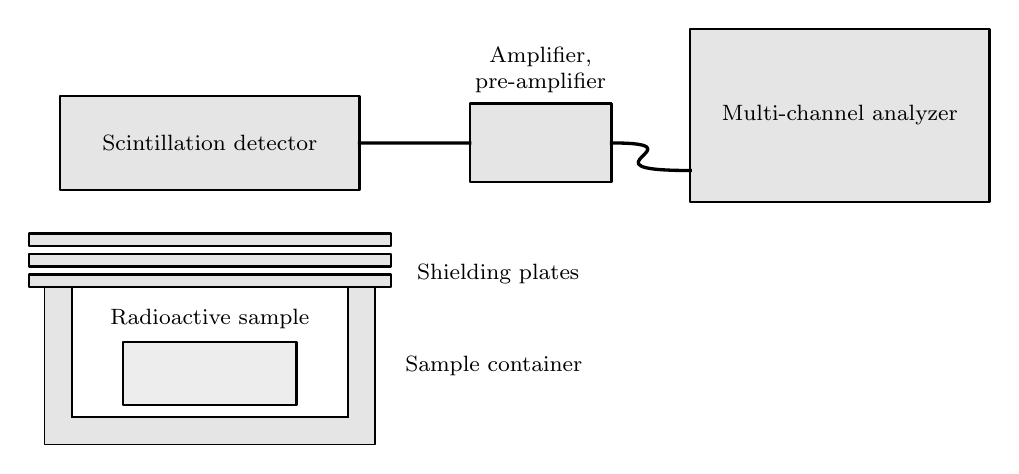
\begin{tikzpicture}[
      line cap=rect, line join=round, >=Latex,
      thick, font=\footnotesize
    ]

    % ------------------ Layout ------------------
    \def\containerWidth{4.2}
    \def\containerHeight{2.0}
    \def\wallThick{0.35}

    \def\shieldWidth{4.6}
    \def\shieldHeight{0.16}
    \def\shieldSep{0.10}

    \def\detW{3.8}
    \def\detH{1.2}
    \def\detGap{0.45}

    \def\mcaX{8.0}
    \def\mcaW{3.8}
    \def\mcaH{2.2}

    % ------------------ U-shaped container (union of three
    % rectangles + inner and outer borders) ------------------
    \fill[black!10] (-\containerWidth/2, 0) rectangle ++(\wallThick,
    \containerHeight);
    \fill[black!10] (-\containerWidth/2, 0) rectangle
    ++(\containerWidth, \wallThick);
    \fill[black!10] ( \containerWidth/2-\wallThick, 0) rectangle
    ++(\wallThick, \containerHeight);

    \draw[black, line width=0.6pt]
    (-\containerWidth/2, \containerHeight) --
    (-\containerWidth/2, 0) --
    (\containerWidth/2, 0) --
    (\containerWidth/2, \containerHeight);

    \draw[black, line width=0.6pt]
    (-\containerWidth/2+\wallThick, \wallThick) --
    (-\containerWidth/2+\wallThick, \containerHeight);
    \draw[black, line width=0.6pt]
    (\containerWidth/2-\wallThick, \wallThick) --
    (\containerWidth/2-\wallThick, \containerHeight);
    \draw[black, line width=0.6pt]
    (-\containerWidth/2+\wallThick, \wallThick) --
    (\containerWidth/2-\wallThick, \wallThick);

    % ------------------ Radioactive sample ------------------
    \def\sampleW{2.2}
    \def\sampleH{0.8}
    \pgfmathsetmacro{\sampleY}{\wallThick+0.15}
    \draw[fill=black!7, draw=black] (-\sampleW/2,\sampleY) rectangle
    ++(\sampleW,\sampleH);
    \node[above=1pt] at (0,\sampleY+\sampleH) {Radioactive sample};

    % ------------------ Shielding plates ------------------
    \foreach \i in {0,1,2} {
      \pgfmathsetmacro{\y}{\containerHeight + \i*(\shieldHeight+\shieldSep)}
      \filldraw[fill=black!10, draw=black] (-\shieldWidth/2,\y)
      rectangle ++(\shieldWidth,\shieldHeight);
    }
    \node[anchor=west] at (\shieldWidth/2+0.2, \containerHeight +
    \shieldHeight) {Shielding plates};

    % ------------------ Scintillation detector ------------------
    \pgfmathsetmacro{\detY}{\containerHeight +
    3*(\shieldHeight+\shieldSep) + \detGap}
    \filldraw[fill=black!10, draw=black] (-\detW/2,\detY) rectangle
    ++(\detW,\detH);
    \node at (0,\detY+0.5*\detH) {Scintillation detector};

    % ------------------ Amplifier ------------------
    \def\ampW{1.8}
    \def\ampH{1.0}
    \pgfmathsetmacro{\ampX}{4.2}
    \pgfmathsetmacro{\ampY}{\detY + 0.1}
    \filldraw[fill=black!10, draw=black] (\ampX-\ampW/2,\ampY)
    rectangle ++(\ampW,\ampH);
    \node[above, align=center] at (\ampX,\ampY+\ampH)
    {Amplifier,\\pre-amplifier};

    % ------------------ MCA ------------------
    \filldraw[fill=black!10, draw=black] (\mcaX-\mcaW/2,\detY-0.15)
    rectangle ++(\mcaW,\mcaH);
    \node at (\mcaX, \detY-0.15+\mcaH/2) {Multi-channel analyzer};

    % ------------------ Signal path ------------------
    \draw[very thick]
    (\detW/2, \detY+0.5*\detH)
    .. controls +(1.0,0.0) and +(-1.0,0.0) ..
    (\ampX-\ampW/2, \ampY+\ampH/2);

    \draw[very thick]
    (\ampX+\ampW/2, \ampY+\ampH/2)
    .. controls +(1.2,0.0) and +(-1.5,0.0) ..
    (\mcaX-\mcaW/2, \detY+0.25);

    % ------------------ Signal label ------------------
    \pgfmathsetmacro{\signalMidX}{(\detW/2 + \mcaX - \mcaW/2)/2}

    % ------------------ Helper labels ------------------
    \node[anchor=west] at (\containerWidth/2+0.25,
    \containerHeight/2) {Sample container};

  \end{tikzpicture}

  \caption{A schematic of the experimental apparatus. A radioactive
    sample is placed in a container shielding the
    experimentalist from radiation. Plates of shielding material are
    placed between the
    sample and a scintillation detector, which converts gamma rays into voltage
    signals. A pre-amplifier and amplifier pair adjust the signal to
    suitable parameters for the MCA: the voltage is set to an
    expected operation range
  and voltage pulses are shaped to be well-defined on an oscilloscope.}
  \label{fig:apparatus}
\end{figure}

\begin{figure}[H]
  \centering
  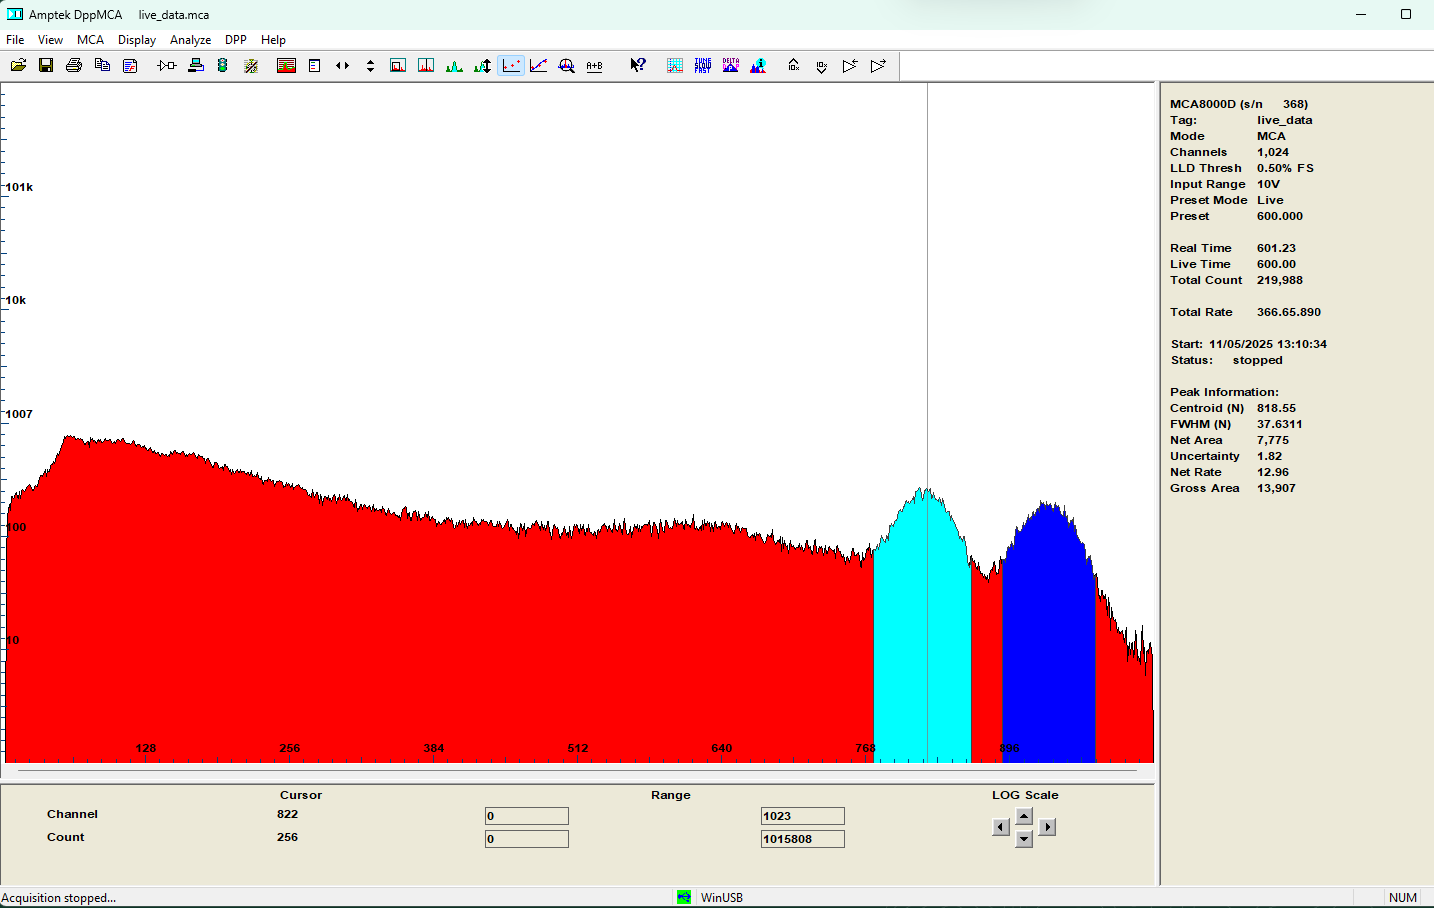
\includegraphics[width=0.8\textwidth]{../spect.png}
  \caption{A spectrum of frequency versus channel number (energy
    proxy) as displayed by the MCA for Cobalt-60 with no shielding material.
    Note the two emission peaks of
  Cobalt-60, highlighted in light blue and dark blue.}
  \label{fig:spectrum}
\end{figure}

\section{Results}

\begin{table}[H]
  \centering
  \begin{tabular}{|c|c|c|}
    \hline
    Peak 1 (counts) & Peak 2 (counts) & Thickness (cm) \\
    \hline
    $225 \pm 15$ & $140 \pm 12$ & $0.00$ \\
    $211 \pm 15$ & $143 \pm 12$ & $1.30 \pm 0.10$ \\
    $164 \pm 13$ & $152 \pm 12$ & $2.61 \pm 0.20$ \\
    $137 \pm 12$ & $103 \pm 10$ & $4.0 \pm 0.3$ \\
    $125 \pm 11$ & $90 \pm 10$ & $5.3 \pm 0.4$ \\
    $111 \pm 11$ & $87 \pm 9$ & $6.6 \pm 0.5$ \\
    $77 \pm 9$ & $56 \pm 7$ & $7.9 \pm 0.6$ \\
    \hline
  \end{tabular}
  \label{tab:al_data}
  \caption{Gamma emission counts for aluminum shielding material at
    the peak 1 (1.1732 MeV) and peak 2 (1.3325 MeV) \cite{nudat} of
    Cobalt-60 for
    different shielding material thicknesses. Counts were accrued
    in a 10-minute
  interval for each thickness.}
\end{table}

\begin{table}[H]
  \centering
  \begin{tabular}{|c|c|c|}
    \hline
    Peak 1 (counts) & Peak 2 (counts) & Thickness (cm) \\
    \hline
    $340 \pm 18$ & $261 \pm 16$ & $0.00$ \\
    $264 \pm 16$ & $187 \pm 14$ & $0.51 \pm 0.10$ \\
    $162 \pm 13$ & $155 \pm 12$ & $1.05 \pm 0.20$ \\
    $128 \pm 11$ & $108 \pm 10$ & $1.60 \pm 0.30$ \\
    $76 \pm 9$ & $84 \pm 9$ & $2.10 \pm 0.40$ \\
    $70 \pm 8$ & $53 \pm 7$ & $2.70 \pm 0.50$ \\
    $54 \pm 7$ & $36 \pm 6$ & $3.20 \pm 0.60$ \\
    \hline
  \end{tabular}
  \caption{Gamma emission counts for lead shielding material at
    the peak 1 (1.1732 MeV) and peak 2 (1.3325 MeV) of Cobalt-60 for
    different shielding material thicknesses. Counts were accrued
    in a 10-minute
  interval for each thickness.}
  \label{tab:pb_data}
\end{table}

\begin{figure}[H]
  \centering
  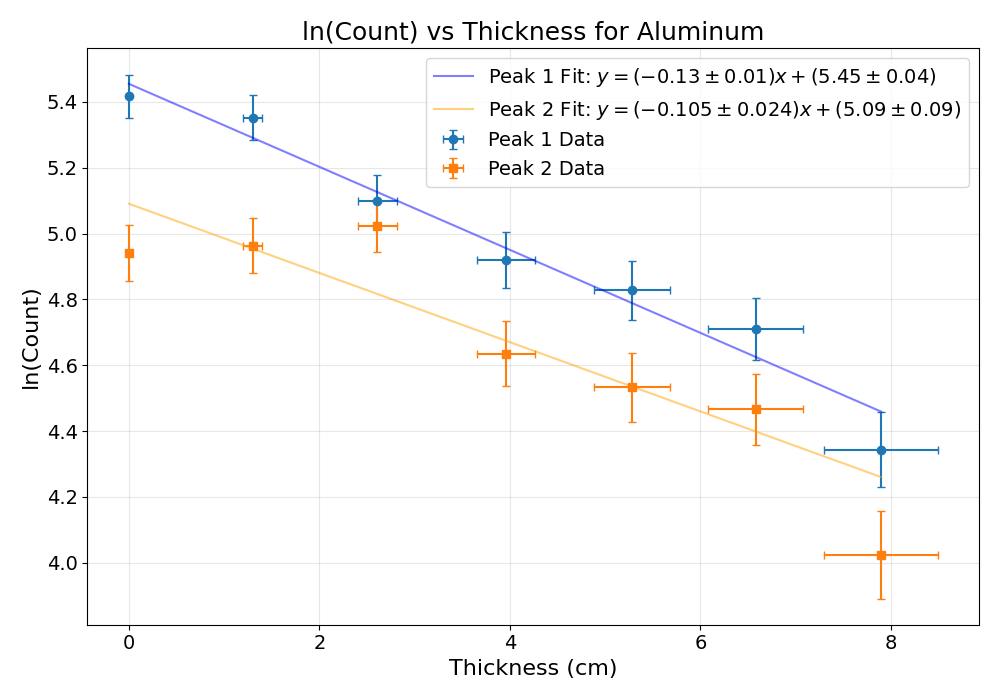
\includegraphics[width=0.8\textwidth]{../aluminum_attenuation.png}
  \caption{A plot of the natural logarithm of the peak count versus
    the thickness of the shielding material for aluminum, corresponding
    to Equation \eqref{eq:lin_reg} and created with data derived from
    Table \ref{tab:al_data}. Data for peak 1 is plotted in blue and
    data for peak 2 is plotted in orange. The slope corresponding to
    the least squares fit provides $-\alpha$, from which $\mu$ is
  derived. Origin not shown.}
  \label{fig:aluminum_attenuation}
\end{figure}

\begin{figure}[H]
  \centering
  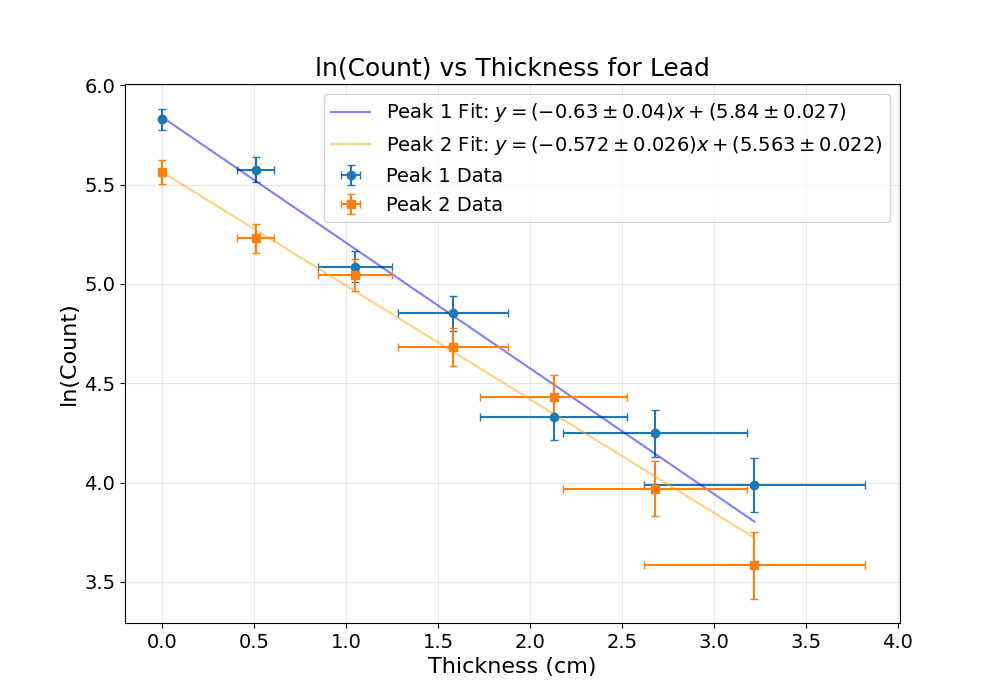
\includegraphics[width=0.8\textwidth]{../lead_attenuation.png}
  \caption{A plot of the natural logarithm of the peak count versus
    the thickness of the shielding material for lead, corresponding
    to Equation \eqref{eq:lin_reg} and created with data derived from
    Table \ref{tab:pb_data}. Data for peak 1 is plotted in blue and
    data for peak 2 is plotted in orange. The slope corresponding to
    the least squares fit provides $-\alpha$, from which $\mu$ is
  derived. Origin not shown.}
  \label{fig:lead_attenuation}
\end{figure}

The data of tables \ref{tab:al_data} and \ref{tab:pb_data} are plotted in
Figures \ref{fig:aluminum_attenuation} and
\ref{fig:lead_attenuation}, respectively. Using a linear
regression fit, slopes corresponding to $-\alpha$ are found, from which
experimental values
for the
mass attenuation
coefficient $\mu = \frac{\alpha}{\rho}$ for peaks 1 and 2 for
aluminum and lead are derived. These values are reported in Table
\ref{tab:mu_values}, along with
discrepancies from the accepted values of $\mu$ obtained from the
public NIST database via Equation \eqref{eq:lin_interp} \cite{nist-gen,
nist-pb, nist-al}.

\begin{table}[H]
  \centering
  \begin{tabular}{|c|c|c|c|}
    \hline
    Experiment & Measured $\mu$ (m$^2$/kg) & Accepted $\mu$
    (m$^2$/kg) & Discrepancy ($\sigma$) \\
    \hline
    1.1732 MeV Peak, Pb & $0.0056 \pm 0.0003$ & $0.00625$ & $2.2$ \\
    1.3325 MeV Peak, Pb & $0.00504 \pm 0.00023$ & $0.00566$ & $2.7$ \\
    1.1732 MeV Peak, Al & $0.0047 \pm 0.0004$ & $0.00570$ & $2.8$ \\
    1.3325 MeV Peak, Al & $0.0039 \pm 0.0009$ & $0.00533$ & $1.6$ \\
    \hline
  \end{tabular}
  \caption{Experimental values of the mass attenuation coefficient $\mu$ for
  peaks 1 and 2 for aluminum and lead, respectively.}
  \label{tab:mu_values}
\end{table}

\section{Discussion and Conclusion}

Significant deviation from the accepted values of $\mu$ for both
emission peaks
and shielding materials is observed; for most trials, discrepancies
are above $2\sigma$. Primary causes for these discrepancies might include
a lack of thorough
shielding of the scintillation detector from external radiation,
plates of shielding material
that were not adequately large or aligned above the container cavity,
and irregularities (local noise) in the peaks collected by the MCA.
Despite an expected
exponential relationship between the number of gamma rays collected
by the scintillation
detector and the thickness of the shielding material, significant
qualitative deviations of the aluminum data points from a linear
trend are noted in Figure \ref{fig:aluminum_attenuation}. A more
thorough conduction of the experiment would involve larger
plates to guarantee full coverage of the cavity and an average of the
peak values per thickness and material to reduce the impact of peak
irregularities.

\bibliographystyle{plain}
\bibliography{references}

\end{document}
